\chapter{DASAR TEORI}\label{dasar-teori}

%---- NEW
%---- SECTION

\section{Parameter Akustika pada Instrumen Musik}
Bunyi (termasuk bunyi instrumen musik) adalah energi yang dihasilkan oleh getaran suatu objek, di mana energi ini merambat pada medium dalam bentuk gelombang. Dari definisi ini diketahui bahwa bunyi dapat terjadi karena dua hal, yaitu objek yang bergetar dan medium perambatan gelombang. Gelombang bunyi dapat merambat melalui medium padat dan fluida. Ketika sebuah instrumen musik bergetar, getarannya mengguncangkan udara dan membuat tekanan udara sekitar berfluktuasi \cite{handbookAcoustic}. Bunyi yang dihasilkan instrumen musik ini memiliki berbagai parameter yang dapat diukur nilainya. Dalam konteks masalah pementasan musik, terdapat tiga parameter objektif yang penting untuk dianalisis, yaitu TTB, frekuensi, dan direktivitas. \par

\subsection{Tingkat Tekanan Bunyi}
Seperti yang telah dijelaskan, bunyi merupakan fluktuasi tekanan. Bunyi dapat dirasakan karena sistem pendengaran manusia peka terhadap perubahan tekanan. Gelombang bunyi bukanlah udara yang mengalir, namun fluktuasi tekanan udara yang berubah-ubah akibat adanya getaran objek. Dari sini diketahui bahwa perambatan bunyi membutuhkan medium karena fluktuasi tekanan dapat terjadi ketika sudah adanya tekanan udara sekitar. Secara matematis, fluktuasi tekanan didefinisikan dengan
\begin{equation}
    p_T(x,t)=p_0(x,t)+p_1(x,t)
\end{equation}
di mana $p_0$ adalah tekanan fluida sekitar, $p_1$ adalah fluktuasi tekanan, dan $p_T$ adalah tekanan total. Tekanan atmosfer udara bumi bernilai 1 atm = 1,013 $\times$ 10\textsuperscript{5} Pa \cite{handbookAcoustic}. \par 
Secara umum, tekanan bunyi yang dapat dirasakan oleh pendengaran manusia berkisar dari 20 $\mu$Pa sampai dengan sekitar 200 Pa \cite{handbookAcoustic}. Rentang tekanan bunyi yang dapat didengar ini sangatlah luas. Sebagai contoh, tekanan bunyi minimum untuk didengar manusia adalah 20 $\mu$Pa, pada percakapan normal sehari-hari tekanan bunyinya bernilai 0,02 Pa, tekanan bunyi pesawat jet pada jarak 150 m adalah 20 Pa, sedangkan batas tekanan bunyi yang bisa ditolerir rasa sakitnya oleh manusia berada pada nilai 200 Pa. Rentang yang sangat lebar ini sulit untuk direpresentasikan dalam skala linear, karena resolusi interval untuk nilai tekanan bunyi yang rendah akan menjadi sangat buruk. \par
Metode paling tepat untuk merepresentasikan rentang tekanan bunyi adalah dengan menggunakan skala logaritmik. Skala ini mampu memperlihatkan setiap jarak nilai yang bersifat eksponensial dengan lebih jelas. Satuan yang digunakan untuk merepresentasikan nilai dalam skala logaritmik disebut Bel. Bel digunakan untuk menyatakan perbandingan nilai daya dalam skala logaritmik. Karena nilai daya sebanding dengan kuadrat nilai tekanan $\left(P \varpropto p^2\right)$ \cite{handbookAcoustic} maka satuan Bel untuk tekanan bunyi dinyatakan sebagai
\begin{equation}
    \text{SPL Bel} = \log \left(\frac{p}{p_{ref}}\right)^2 = 2 \log \left(\frac{p}{p_{ref}}\right)
\end{equation}
dengan $p$ adalah tekanan bunyi yang diukur dan $p_{ref}$ adalah tekanan bunyi referensi, di mana untuk bunyi di udara nilai yang dijadikan referensi adalah batas tekanan bunyi minimum pendengaran manusia, yaitu 20 $\mu$Pa \cite{handbookAcoustic}. Untuk mendapatkan rentang yang lebih besar, digunakan satuan desibel (dB) yang bernilai $1/10$ Bel. Dengan begitu, nilai tekanan bunyi dalam satuan desibel secara matematis dinyatakan dengan \par 
\begin{equation}
    \text{SPL (dB)} = 20 \log \left(\frac{p}{p_{ref}}\right) \\
    \label{eq:spl-desibel}
\end{equation}

Pada Tabel \ref{tab:hubungan-spl-desibel} diperlihatkan beberapa contoh nilai tekanan sumber bunyi yang dinyatakan dalam [Pa] dan [dB]. Dengan 20 $\mu$Pa sebagai nilai referensi, dapat dilihat bahwa semakin tinggi nilai tekanan bunyinya, jumlah pangkat bilangan dasar 10 pada nilai tekanan bunyi relatif akan semakin bertambah. Dari fakta inilah istilah "Tingkat" pada penyebutan Tingkat Tekanan Bunyi (TTB) berasal \cite{meyer}. \par 
\begin{table}[t!]
    \centering
    \caption{Hubungan antara tekanan bunyi dengan skala desibel untuk beberapa sumber bunyi \cite{ArtikelBukuSPL}.}
    \begin{tabular}{l l l l}
        \hline
        Tekanan Bunyi & Tekanan bunyi & \multirow{2}{4em}{Desibel} & \multirow{2}{8em}{Sumber bunyi} \\
        (Pa) & relatif & & \\
        \hline
        20 & 10\textsuperscript{6} & 120 & Pesawat jet pada jarak 150 m \\
        2 & 10\textsuperscript{5} & 100 & Di dalam gerbong kereta \\
        0,2 & 10\textsuperscript{4} & 80 & Kantor yang berisik \\
        0,02 & 10\textsuperscript{3} & 60 & Percakapan normal \\
        0,002 & 10\textsuperscript{2} & 40 & Perpustakaan umum \\
        0,0002 & 10 & 20 & Suasana kota malam hari \\
        0,00002 & 1 & 0 & Batas minimum pendengaran \\
        \hline
    \end{tabular}
    \label{tab:hubungan-spl-desibel}
\end{table}

\subsection{Frekuensi}
Jumlah fluktuasi tekanan atau getaran udara dalam durasi waktu satu sekon disebut sebagai frekuensi \cite{meyer}. Pada Gambar \ref{fig:gambar-frekuensi} diperlihatkan penggambaran fluktuasi tekanan udara dan analoginya dengan bentuk gelombang transversal. Gambar ini juga menunjukkan rentang mana yang dihitung sebagai satu periode getaran. Satu getaran dihitung ketika tekanan udara telah mengalami puncak tertinggi dan puncak terendah. Secara matematis, frekuensi didefinisikan sebagai
\begin{equation}
    f=\frac{n}{t}=\frac{1}{T}
\end{equation}
di mana $n$ adalah banyaknya getaran, $t$ adalah waktu [detik], dan $T$ adalah periode getaran [detik] \cite{bukuFletcher}. \par
\begin{figure}[t!]
    \centering
    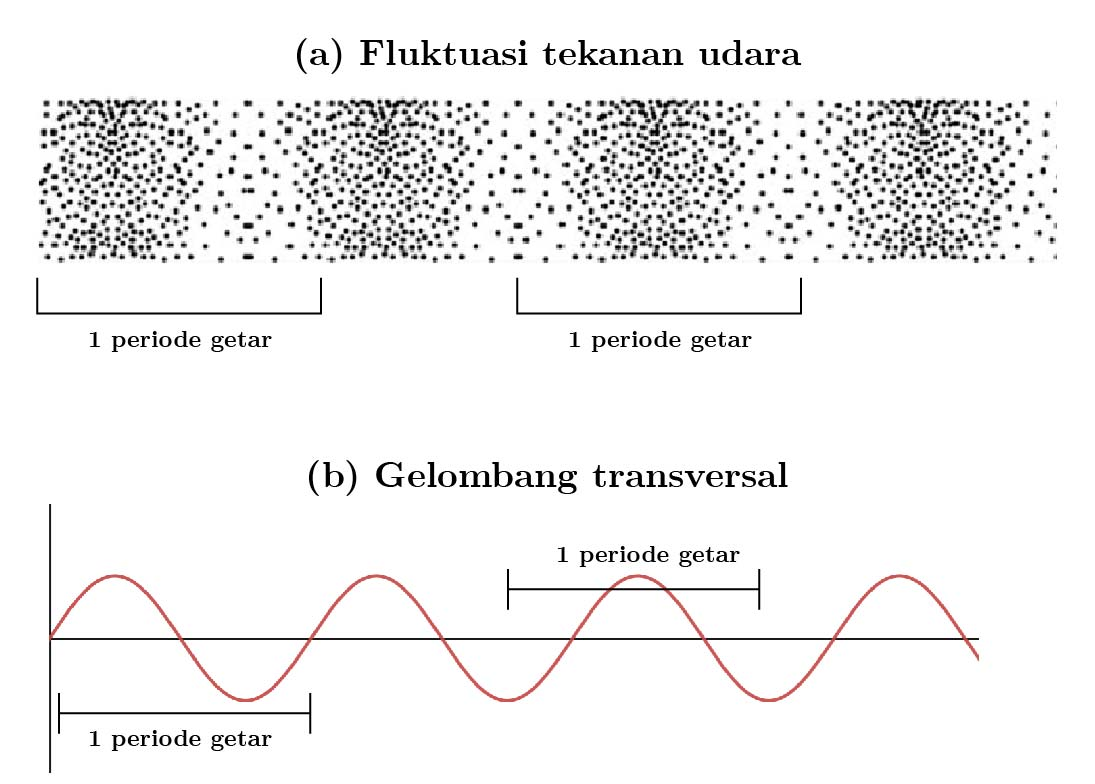
\includegraphics[width=12cm]{Gambar/gambar-frekuensi-03.jpg}
    \caption{(a) Penggambaran fluktuasi tekanan udara dan analoginya dengan (b) gelombang transversal \cite{handbookAcoustic}.}
    \label{fig:gambar-frekuensi}
\end{figure}
Banyaknya getaran setiap satu detik dinyatakan dalam satuan Hz ("Hertz"). Frekuensi getaran yang dapat dirasakan pendengaran manusia berada pada rentang 16 Hz--20 kHz \cite{meyer}. Dalam musik, tingkatan nada atau \textit{pitch} disebabkan oleh perbedaan frekuensi. Sebagai contoh, nada referensi musik A\textsubscript{4} memiliki frekuensi 440 Hz. Pada Tabel \ref{tab:frekuensidanNada} diperlihatkan berbagai nilai frekuensi dan hubungannya dengan nada pada musik. \par
\begin{table}[b!]
    \centering
    \caption{Hubungan nilai frekuensi dengan nada musik \cite{meyer}.}
    \begin{tabular}{c l}
        \hline
        Frekuensi (Hz) & Nada \\
        \hline
        16,5 & C\textsubscript{0} kunci C pada organ 32' \\
        33 & C\textsubscript{1} senar-C dari 5 senar contrabass \\
        66 & C\textsubscript{2} senar-C pada cello \\
        131 & C\textsubscript{3} senar-C pada viola \\
        262 & C\textsubscript{4} C terendah pada biola \\
        524 & C\textsubscript{5} C tenor tinggi \\
        1.047 & C\textsubscript{6} C sopran tinggi \\
        2.093 & C\textsubscript{7} C biola tertinggi \\
        4.185 & C\textsubscript{8} C tertinggi piccolo \\
        \hline
    \end{tabular}
    \label{tab:frekuensidanNada}
\end{table}

\subsection{Direktivitas Bunyi}
Sumber bunyi paling sederhana adalah sumber bunyi berbentuk titik, yang mana sumber titik ini diibaratkan bola berdenyut dengan jari-jari mendekati nol \cite{bukuFletcher}. Sumber bunyi ini disebut sumber bunyi monopol, yaitu sumber bunyi yang meradiasikan bunyi secara merata ke segala arah (omnidireksional). Secara matematis, tekanan bunyi dari sebuah titik dengan jari-jari $a$ yang berdenyut dengan frekuensi $\omega$ dinyatakan sebagai berikut
\begin{equation}
    p(r)=\frac{j\omega \rho}{4 \pi r}Qe^{-jkr}
    \label{eq:monopol}
\end{equation}
di mana $r$ adalah jarak radius perambatan bunyi, $\rho$ adalah densitas medium, $k$ adalah bilangan gelombang, dan $Q$ adalah debit udara yang berdenyut \cite{bukuFletcher}. Persamaan ini hanya berlaku untuk titik berdenyut dengan jari-jari sangat kecil mendekati 0, sehingga $ka \ll 1$. Pada Gambar \ref{fig:monopol} diperlihatkan penggambaran dari sumber bunyi monopol. \par
\begin{figure}[t!]
    \centering
    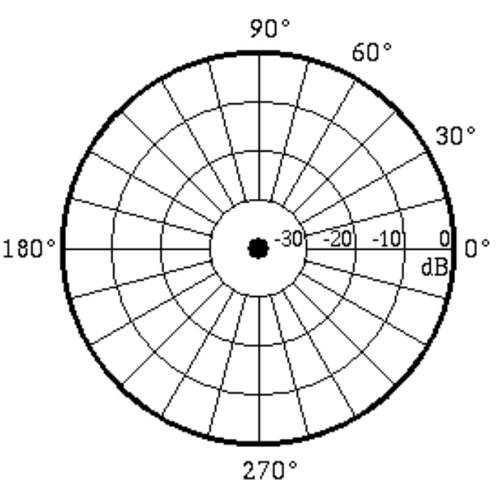
\includegraphics[width=5 cm]{Gambar/monopol.jpg}
    \caption{Visualisasi tekanan bunyi sumber monopol pada diagram polar \cite{danRussel-pole}.}
    \label{fig:monopol}
\end{figure}
Apabila terdapat dua buah sumber monopol identik berdekatan dengan fase yang berlawanan maka sumber bunyi ini disebut sebagai sumber dipol \cite{bukuFletcher}. Pada Gambar \ref{fig:dipol-dobelMonopol} diperlihatkan sumber dipol yang terdiri dari dua sumber monopol identik dengan debit denyut $\pm Q$ dan terpisah dengan jarak $dz$.
\begin{figure}[t!]
    \centering
    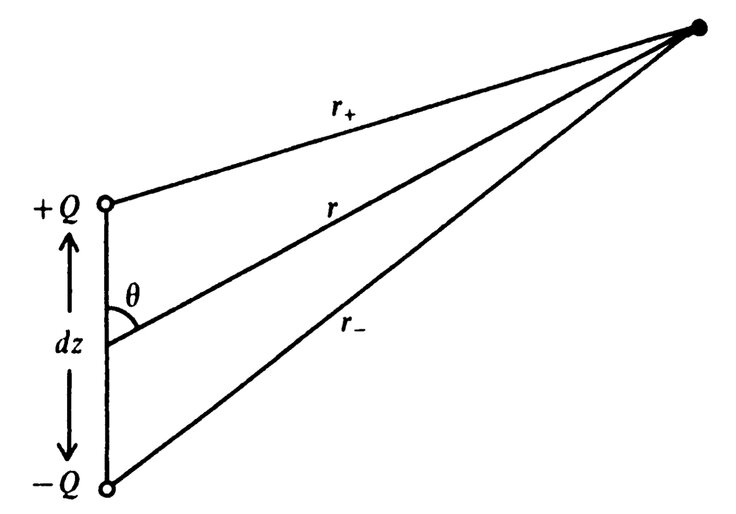
\includegraphics[width = 8 cm]{Gambar/dipol-dobelMonopol.jpg}
    \caption{Sumber bunyi dipol. Untuk nilai $dz \rightarrow 0$, $Q \rightarrow \infty$, nilai momen dipol sebesar $\mu = Q \, dz$ \cite{bukuFletcher}.}
    \label{fig:dipol-dobelMonopol}
\end{figure}
Secara matematis, nilai tekanan bunyi yang berasal dari sumber dipol tersebut dapat dinyatakan dengan 
\begin{equation}
    p(r,\theta)=\frac{\omega^2 \rho}{4 \pi c r}\left(1+\frac{1}{jkr}\right)e^{-jkr}\mu\cos\theta
    \label{eq:dipol}
\end{equation}
di mana $c$ adalah cepat rambat bunyi, $r$ adalah jarak antara pusat dipol dengan titik ukur, dan $\theta$ adalah sudut yang terbentuk dari titik ukur dengan sumber dipol \cite{bukuFletcher}. \par 
\begin{figure}[b!]
    \centering
    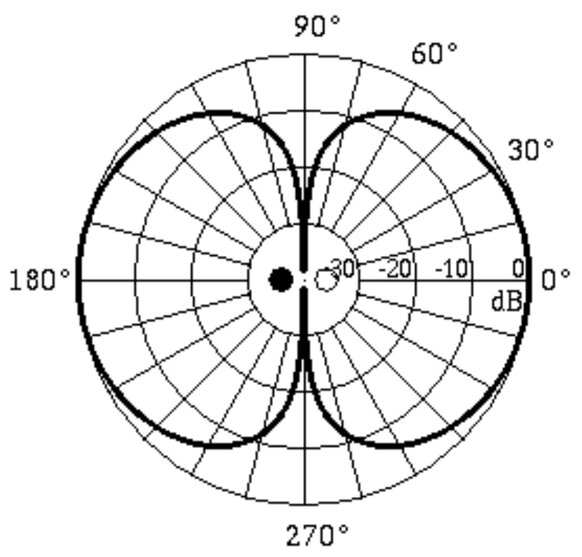
\includegraphics[width= 5 cm]{Gambar/dipol.jpg}
    \caption{Visualisasi tekanan bunyi sumber dipol pada diagram polar \cite{danRussel-pole}.}
    \label{fig:dipol}
\end{figure}
Karena nilai fase dua sumber monopol penyusun sumber dipol tersebut saling berlawanan, akibatnya udara di sekitar kedua sumber monopol akan bergetar bolak-balik sehingga menghasilkan bunyi. Oleh sebab itu, sumber bunyi yang bergetar bolak-balik dapat dikatakan berperilaku seperti sumber bunyi dipol \cite{danRussel-pole}, termasuk senar yang bergetar. Pada Gambar \ref{fig:dipol} diperlihatkan pola sebaran tekanan bunyi sebuah sumber dipol. Dari pola tersebut dapat diamati bahwa sumber dipol tidak meradiasikan bunyi secara merata ke segala arah. Terdapat area di mana bunyi secara merata diradiasikan dan ada area di mana tidak terdapat tekanan bunyi. \par
Faktanya, setiap instrumen musik tidak menghasilkan bunyi dengan nilai yang sama ke segala arah. Setiap frekuensi, pada setiap arah rambat bunyi memiliki nilai TTB yang berbeda-beda. Perbedaan nilai TTB berdasarkan arah rambat bunyi ini disebut sebagai karakteristik direksional atau direktivitas \cite{meyer}. Pada Gambar \ref{fig:direktivitas-oboe} diperlihatkan pola direktivitas dari oboe untuk berbagai nilai frekuensi. Dapat diamati bahwa untuk nilai frekuensi yang berbeda, nilai TTB untuk setiap arah rambat bunyi oboe juga berbeda. \par
\begin{figure}[t!]
    \centering
    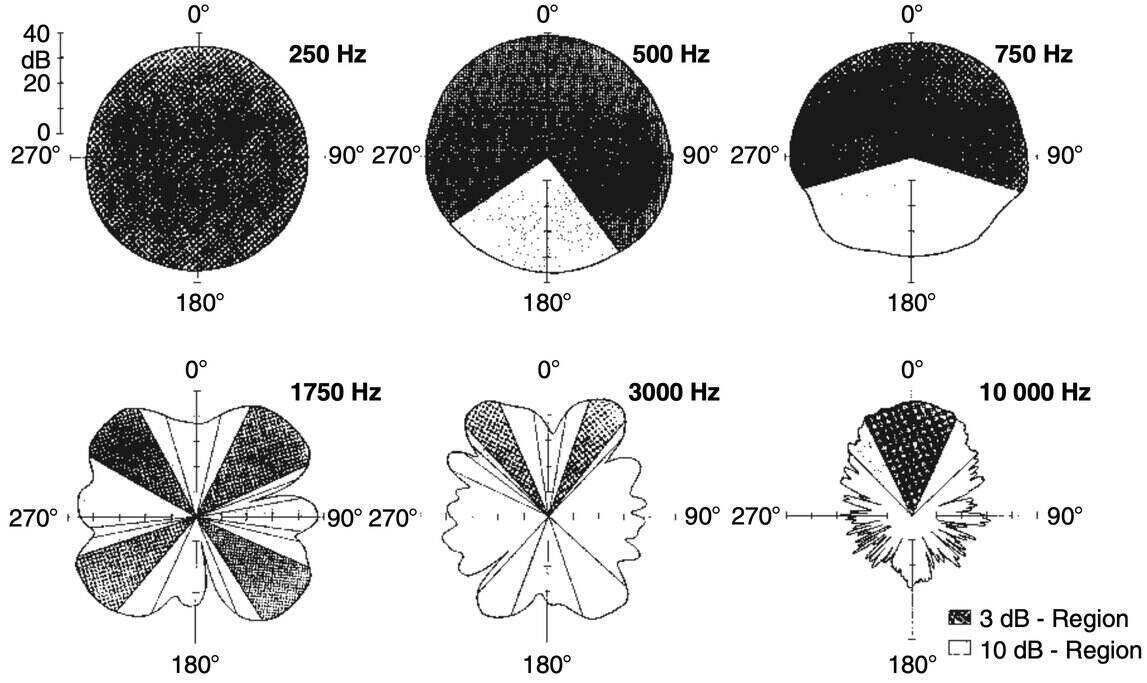
\includegraphics[width=11cm]{Gambar/direktivitas-oboe.jpg}
    \caption{Pola direktivitas oboe untuk beberapa nilai frekuensi. Arah $0^\circ$ menunjukkan arah axis oboe \cite{meyer}.}
    \label{fig:direktivitas-oboe}
\end{figure}


%--- NEW
%--- SECTION

\section{Visualisasi}
Alur proses representasi kumpulan data mentah menjadi sebuah tampilan interaktif kepada pengguna ditunjukkan pada Gambar \ref{fig:visual-pipeline}. Pada tahap awal, data mentah diproses menjadi sesuatu yang berguna untuk sistem visualisasi \cite{buku_visual}. Tujuan utama dari tahap ini adalah memetakan data mentah supaya dapat diolah dengan komputer. Pada tahap ini juga dilakukan validasi dari data yang didapat, seperti nilai yang hilang, kesalahan masukan, dan ukuran data yang terlalu besar diperbaiki pada tahap ini. \par
Setelah data mentah benar-benar bersih, proses dilanjutkan dengan penentuan metode representasi visual. Proses ini dapat meliputi pemetaan geometri, warna, dan suara. Dalam penentuan metode visualisasi data, terdapat dua nilai yang sangat krusial, yaitu keekspresifan dan keefektifan \cite{buku_visual}. \par 
\begin{figure}[t!]
    \centering
    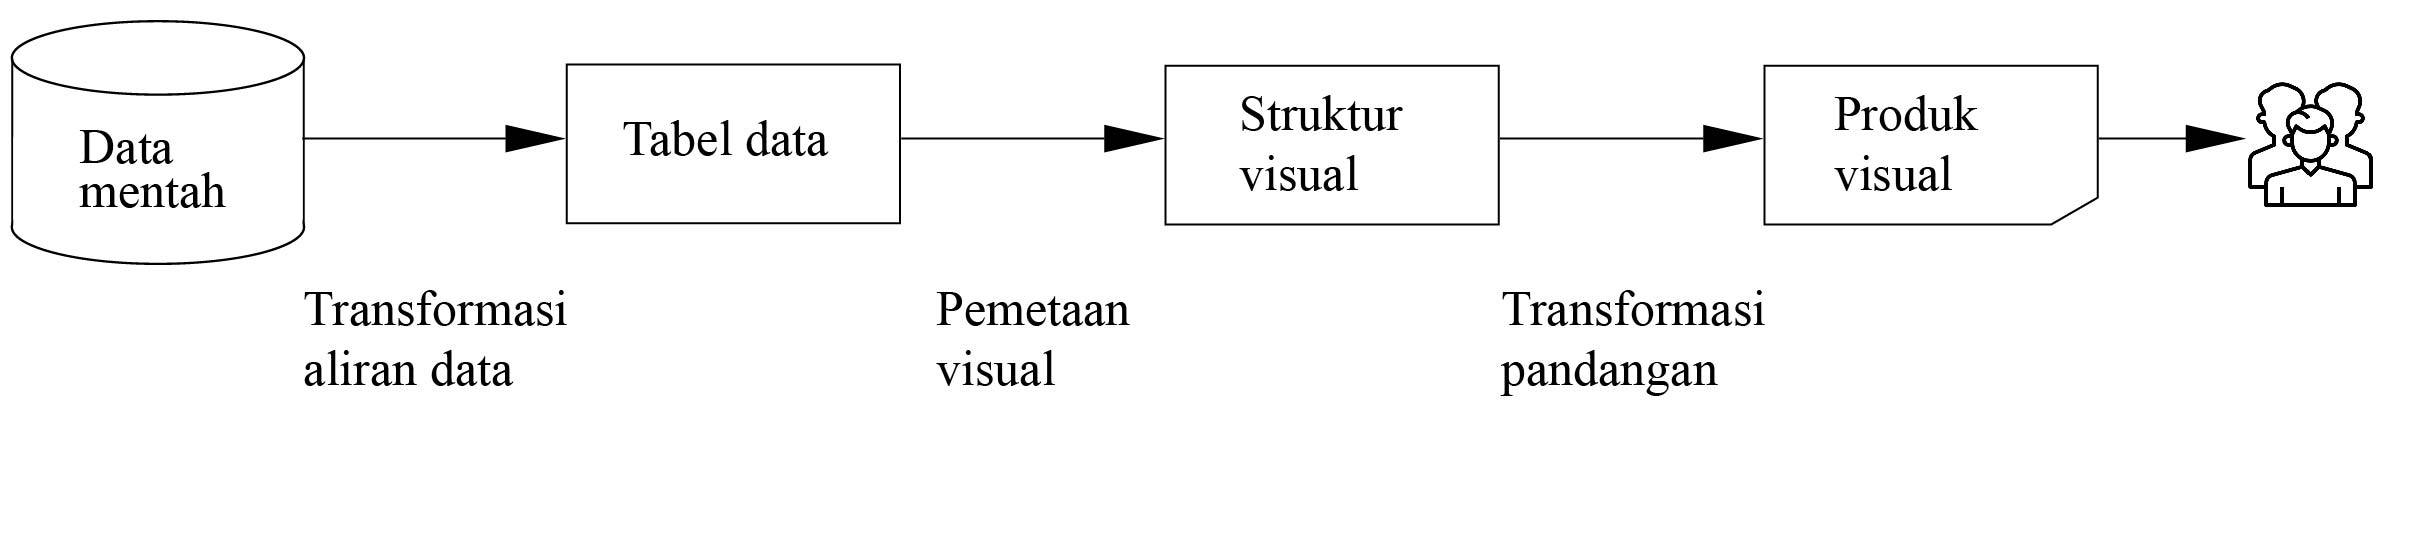
\includegraphics[width = 13 cm]{Gambar/visualisasi-pipeline.jpg}
    \caption{Alur proses visualisasi \cite{buku_visual}.}
    \label{fig:visual-pipeline}
\end{figure}
\begin{enumerate}
    \item Visualisasi dikatakan ekspresif ketika menampilkan keseluruhan data secara utuh dan terfokus pada informasi yang hendak disampaikan. Untuk mengukur tingkat keekspresifan, digunakan nilai $M_{\text{exp}}$ yaitu rasio antara informasi yang ditampilkan kepada pengguna dengan keseluruhan informasi. Nilai ini berkisar pada rentang $0 \leq M_{\text{exp}} \leq 1$. Nilai $M_{\text{exp}}=1$ menunjukkan keekspresifan visualisasi yang ideal, sedangkan nilai $M_{\text{exp}} < 1$ menyatakan sistem visualisasi belum menampilkan keseluruhan informasi yang seharusnya. Pada beberapa kasus, nilai keekspresifan dapat bernilai lebih dari 1. Hal ini terjadi apabila sistem menampilkan informasi tambahan selain informasi yang direncanakan, sehingga berpotensi mengganggu konsentrasi pengguna.
    \item Visualisasi dikatakan efektif apabila dapat diinterpretasi dengan akurat dan cepat. Keefektifan mengukur secara spesifik "biaya" dari persepsi informasi. Nilai keefektifan diukur dengan $M_{\text{eff}}$, yaitu sebuah rasio yang mirip dengan nilai keekspresifan, namun sedikit lebih kompleks. Nilai ini diukur dari waktu interpretasi dan waktu \textit{render}. Waktu interpretasi adalah durasi yang dibutuhkan pengguna untuk memproses informasi yang ditampilkan. Proses ini meliputi ditangkapnya objek visual oleh indera manusia sampai selesai dipahami oleh persepsi otak manusia. \textit{Rendering} adalah proses sistem visualisasi untuk menampilkan informasi sesuai konsep yang direncanakan. Proses ini adalah tahap ketiga dari alur proses visualisasi. Durasi yang dibutuhkan untuk menampilkan ini disebut sebagai waktu \textit{render}. Untuk sistem visualisasi berbentuk fisik atau visualisasi data kecil, nilai keefektifan ditentukan hanya berdasarkan waktu interpretasi, karena biasanya proses \textit{rendering} telah selesai sehingga waktu \textit{render} dihitung sangat cepat. Ketika waktu interpretasi meningkat, baik karena data semakin kompleks ataupun peningkatan ukuran data, nilai $M_{\text{eff}}$ akan berkurang. Nilai keefektifan didefinisikan dengan \begin{equation}
        M_\text{eff}=1/\left(1+\text{interpret}+\text{render}\right)
    \end{equation} dengan $0 < M_{\text{eff}}\leq 1$. Semakin besar nilai $M_{\text{eff}}$, visualisasi dikatakan semakin efektif.
\end{enumerate}

Tahap terakhir adalah proses \textit{rendering} atau menampilkan. Pada tahap ini konsep visualisasi direalisasikan menjadi bentuk tampak sesuai yang dikehendaki. Proses ini lebih banyak melibatkan pemodelan menggunakan komputer. Parameter objek visual seperti bayangan pada objek 3D, warna objek, dan transformasi perangkat (contoh: pencetakan) dikerjakan pada tahap ini. Hasil akhir tahap \textit{rendering} adalah berupa produk yang dapat ditampilkan kepada pengguna. \par 

\subsection{Dasar Visualisasi}
Pada Gambar \ref{fig:clef} diperlihatkan sebuah simbol yang dapat dengan mudah dikenali, yaitu \textit{treble clef}, sedangkan pada Gambar \ref{fig:direktivitas-kompleks} diperlihatkan representasi data direktivitas \bundengan yang kompleks. Sebuah gambar dapat dengan mudah dikenali banyak orang karena gambar tersebut banyak dilibatkan dalam pengalaman manusia. Simbol \textit{treble clef} dapat dengan mudah dikenali artinya karena digunakan pada notasi musik, sedangkan untuk memahami representasi data direktivitas \bundengan diperlukan perhatian yang lebih. Sebelum memahami makna keseluruhan dari data direktivitas yang ditampilkan, pengguna terlebih dahulu perlu mengerti arti dari sumbu mendatar dan sumbu tegak, serta hubungan antar keduanya. Setelah itu, pengguna perlu mengerti arti dari perbedaan warna yang ditampilkan. Ketika pengguna sudah mengetahui hubungan antar elemen visual yang ada maka pengguna dapat memahami makna dan hubungan setiap variabel yang ditampilkan. \par
\begin{figure}[t!]
    \centering
    \subfigure[]{\label{fig:clef}
\includegraphics[width=43mm]{Gambar/clef.jpg}}
    \hspace{1cm}
    \subfigure[]{\label{fig:direktivitas-kompleks}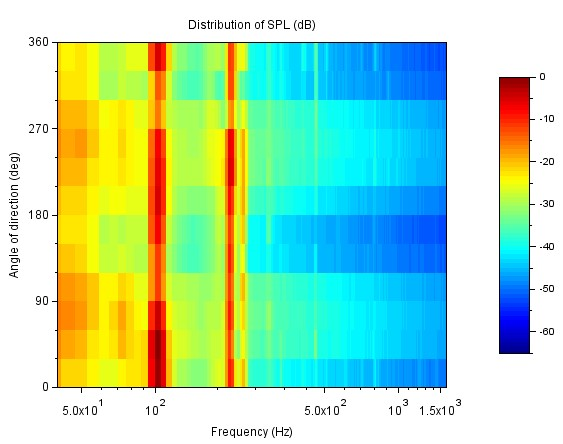
\includegraphics[width=63mm]{Gambar/senar3yangA.jpg}}
    \caption{Dua tipe produk visual: (a) Simbol dengan arti yang jelas \cite{bukuTeoriMusik} dan (b) representasi data dengan arti yang kompleks \cite{prosidingDirektivitas}.}
\end{figure}
Dapat disimpulkan bahwa Gambar \ref{fig:clef} dapat dipahami dalam satu langkah, sedangkan untuk memahami Gambar \ref{fig:direktivitas-kompleks} dibutuhkan dua langkah \cite{buku_visual}. Pada langkah pertama, elemen utama pada gambar diidentifikasi dengan bantuan memori jangka panjang. Gambar \ref{fig:clef} dapat dipahami hanya dengan mengandalkan pengetahuan tentang notasi musik, sedangkan untuk Gambar \ref{fig:direktivitas-kompleks} memori jangka panjang hanya dapat membantu pengguna memahami bahwa representasi data tersebut menggunakan sistem koordinat kartesius. Oleh sebab itu, pemahaman informasi secara utuh terkait Gambar \ref{fig:direktivitas-kompleks} membutuhkan langkah kedua, yaitu dengan menghubungkan konsep koordinat yang telah diketahui dengan elemen lain pada gambar, yaitu spektrum warna. Dengan begitu pengguna akan mulai mengetahui hubungan antar elemen yang merepresentasikan hubungan setiap variabel. \par 
Hal penting terkait representasi data adalah penggunaan elemen visual yang mudah diidentifikasi oleh pengguna \cite{buku_visual}. Jika pengguna tidak memiliki pengetahuan terkait elemen visual yang digunakan maka elemen visual tersebut akan menjadi tidak berguna. Sebagian besar persepsi manusia didorong oleh interpretasi secara fisik, sehingga elemen visual yang bermakna harus memiliki dimensi $x,y,$ dan $z$ yang mudah ditafsirkan \cite{buku_visual}. Selain itu, pola hubungan antar objek grafis yang ditampilkan harus menunjukkan pola pada data. \par
Pada penerapan visualisasi grafis sebagai metode komunikasi diperlukan pemahaman mengenai variabel visualisasi dan sifat-sifatnya \cite{buku_visual}. Penyampaian informasi dalam bentuk tampilan pada dasarnya adalah penyusunan setiap variabel visual menjadi pola tertentu yang dapat dipahami manusia. Sebuah variabel visual yang berdiri sendiri tidak memiliki definisi apapun. Oleh sebab itu, variabel visual perlu melalui proses penyusunan supaya dapat menjadi tampilan yang informatif. \par 
Terdapat delapan variabel visual yang dapat digunakan sebagai penyalur informasi. Delapan variabel ini dapat diatur sedemikian sehingga sesuai dengan kebutuhan dan memaksimalkan keefektifan sistem visualisasi. Berikut adalah delapan variabel visual yang dapat membentuk tampilan informatif pada sistem visualisasi \cite{buku_visual}.
\subsubsection{Posisi}
Penempatan sebuah objek memiliki pengaruh yang sangat besar terhadap informasi mengenai suatu hal. Hal ini karena susunan spasial adalah sesuatu yang pertama kali dibaca oleh otak manusia ketika melihat suatu tampilan yang kompleks. Skema penempatan posisi terbaik adalah meletakkan setiap objek grafis pada posisi unik, sehingga semuanya dapat dilihat dengan jelas tanpa adanya tumpang-tindih antar objek. Penentuan posisi objek grafis juga dipengaruhi oleh variabel yang hendak direpresentasikan. Pemusatan data, distribusi statistik, serta tren pada data dipengaruhi oleh variabel apa yang direpresentasikan. Skala digunakan untuk mengorganisir ruang tampilan dan untuk menghadirkan struktur nilai yang representatif. Yang pertama adalah skala linear, yaitu dengan memetakan setiap data pada rentang nilai tertentu. Yang kedua adalah skala logaritmik, di mana skala ini digunakan untuk memetakan data dengan peningkatan nilai yang eksponensial supaya didapatkan rentang nilai yang lebih mudah diamati.
\subsubsection{Bentuk}
Bentuk adalah konstruksi yang terdiri dari titik, garis, area, dan volume. Perbedaan konstruksi tersebut dapat dijadikan sebagai penanda dua hal yang berbeda ketika menampilkan data. Bentuk-bentuk umum yang digunakan diantaranya adalah lingkaran, persegi, segitiga, bintang, maupun tanda silang. Pertimbangan paling penting dalam pemilihan bentuk adalah seberapa jelas setiap bentuk dapat dibedakan. Hal ini karena pandangan manusia akan sulit untuk mengobservasi sesuatu yang terlihat mirip. Pada Gambar \ref{fig:clef-macammacam} diperlihatkan tiga bentuk \textit{clef} yang dapat dibedakan dengan jelas.
\begin{figure}[t!]
    \centering
    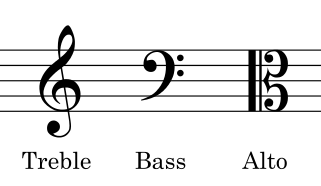
\includegraphics[width=6cm]{Gambar/clef-macam-macam.jpg}
    \caption{Contoh penggunaan bentuk berbeda dalam notasi musik \cite{bukuTeoriMusik}.}
    \label{fig:clef-macammacam}
\end{figure}
Bentuk yang mudah dibedakan ini tentu akan meningkatkan tingkat keefektifan suatu sistem visual.
\subsubsection{Ukuran (Panjang, Luas, dan Volume)}
Variabel visual yang ketiga adalah ukuran. Seberapa besar dan kecilnya objek visual ditentukan dengan ukuran. Perbedaan yang dapat terlihat dalam ruang ini mampu merepresentasikan nilai tertentu. Peningkatan ukuran dapat dijadikan penggambaran peningkatan nilai variabel yang lebih mudah diproses persepsi manusia. 
\subsubsection{Kecerahan}
Kecerahan atau luminansi adalah tingkat hitam-putih suatu objek visual. Kecerahan dapat digunakan untuk dijadikan pembeda untuk beberapa nilai data. Meskipun demikian, kecerahan tidak dapat digunakan sebagai penanda untuk setiap data pada rentang yang lebar secara terpisah. Hal ini karena persepsi manusia tidak dapat membedakan dengan detil tingkat kecerahan suatu objek untuk kemudian diasosiasikan dengan nilai tertentu. Dengan kata lain, kecerahan hanya efektif digunakan untuk merepresentasikan dua nilai yang sangat kontras perbedaannya.
\subsubsection{Warna}
Kecerahan menyatakan seberapa hitam atau seberapa putihnya objek visual, namun sebenarnya yang dinyatakan oleh kecerahan bukanlah warna. Warna dapat didefinisikan dengan dua parameter, yaitu \textit{hue} dan saturasi. Pada Gambar \ref{fig:macam-warna} diperlihatkan pilihan warna dari Microsoft dengan \textit{hue} dinyatakan pada sumbu mendatar dan saturasi pada sumbu tegak. \textit{Hue} menyatakan sesuatu yang kita anggap sebagai warna, yaitu panjang gelombang dari cahaya tampak. Sedangkan saturasi adalah tingkat \textit{hue} relatif terhadap keabu-abuan. Saturasi juga memperlihatkan kemurnian suatu warna yang ditampilkan. Pada penggunaan warna untuk representasi kumpulan informasi, diperlukan pemetaan data pada masing-masing warna. Digunakannya warna sebagai salah satu variabel visual dapat diamati pada Tabel \ref{tab:prosidingDirektivitas}, di mana rentang nilai TTB dinyatakan dalam rentang warna merah sampai biru.
\begin{figure}[t!]
    \centering
    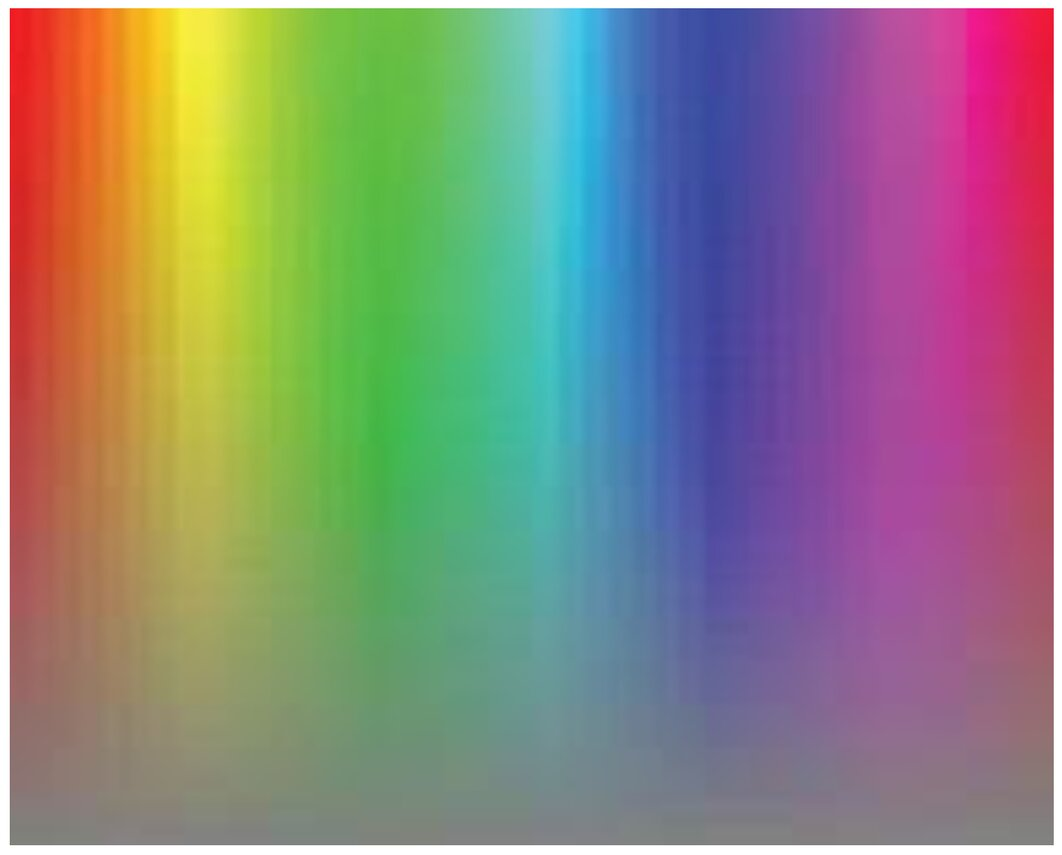
\includegraphics[width=6cm]{Gambar/macam-warna.jpg}
    \caption{\textit{Hue} dan saturasi pada pilihan warna Microsoft \cite{buku_visual}.}
    \label{fig:macam-warna}
\end{figure}
\subsubsection{Orientasi}
Orientasi adalah arah dari sebuah objek visual. Variabel visual ini menyatakan bagaimana sebuah bentuk diputar sehubung dengan informasi yang hendak disampaikan. Perbedaan orientasi tidak selalu dapat digunakan pada semua bentuk objek visual. Penerapan orientasi yang paling baik adalah pada bentuk yang hanya memiliki satu sumbu simetri, seperti segitiga sama kaki. Hal ini karena perbedaan orientasi pada bentuk dengan banyak sumbu simetri tidak terlalu kontras, sehingga persepsi manusia sulit untuk memindai informasi yang hendak disampaikan.
\subsubsection{Tekstur}
Variabel visual yang ketujuh adalah tekstur. Tekstur dapat dikatakan sebagai kombinasi berbagai variabel visual, seperti bentuk, warna, dan orientasi. Garis putus-putus dan titik-titik yang membentuk garis dapat dikategorikan sebagai tekstur. Penggunaan tekstur biasanya diasosiasikan dengan area atau permukaan tertentu. Pada bidang 3D, tekstur dapat berupa perbedaan geometri seperti ketinggian pada permukaan.
\subsubsection{Gerakan}
Variabel visual yang terakhir adalah gerakan. Penerapan umum dari gerakan adalah dengan memvariasikan kecepatan dari perubahan setiap objek visual. Perubahan yang dimaksud dapat berupa perubahan posisi, berkedip, warna, ataupun tingkat gelap-terang. Gerakan dapat berguna untuk menyampaikan informasi karena pandangan manusia akan mengamati perubahan perilaku dari setiap objek visual, tidak hanya perilaku yang mirip, namun perilaku yang bertentangan juga dapat berupa sebuah informasi.


\subsection{Teknik Visualisasi untuk Data Multivariabel}
Berdasarkan buku karya Ward, dkk. \cite{buku_visual}, kumpulan data dapat dikategorikan sebagai data spasial, data geospasial, data temporal, dan data multivariabel. Suatu kumpulan data dikatakan multivariabel jika secara umum tidak ada informasi mengenai kondisi spasial dan waktu tertentu. Data direktivitas \bundengan termasuk dalam kategori data multivariabel, karena data ini tidak menyatakan dengan pasti posisi nilai direktivitas pada titik tertentu dan juga data ini tidak menyatakan nilai direktivitas pada rentang waktu yang spesifik. Kumpulan data jenis ini dapat ditampilkan menggunakan berbagai metode/teknik, baik teknik berbasis titik, garis, area, maupun kombinasi ketiganya. \par 
\subsubsection{Teknik Berbasis Titik}
\begin{figure}[t!]
    \centering
    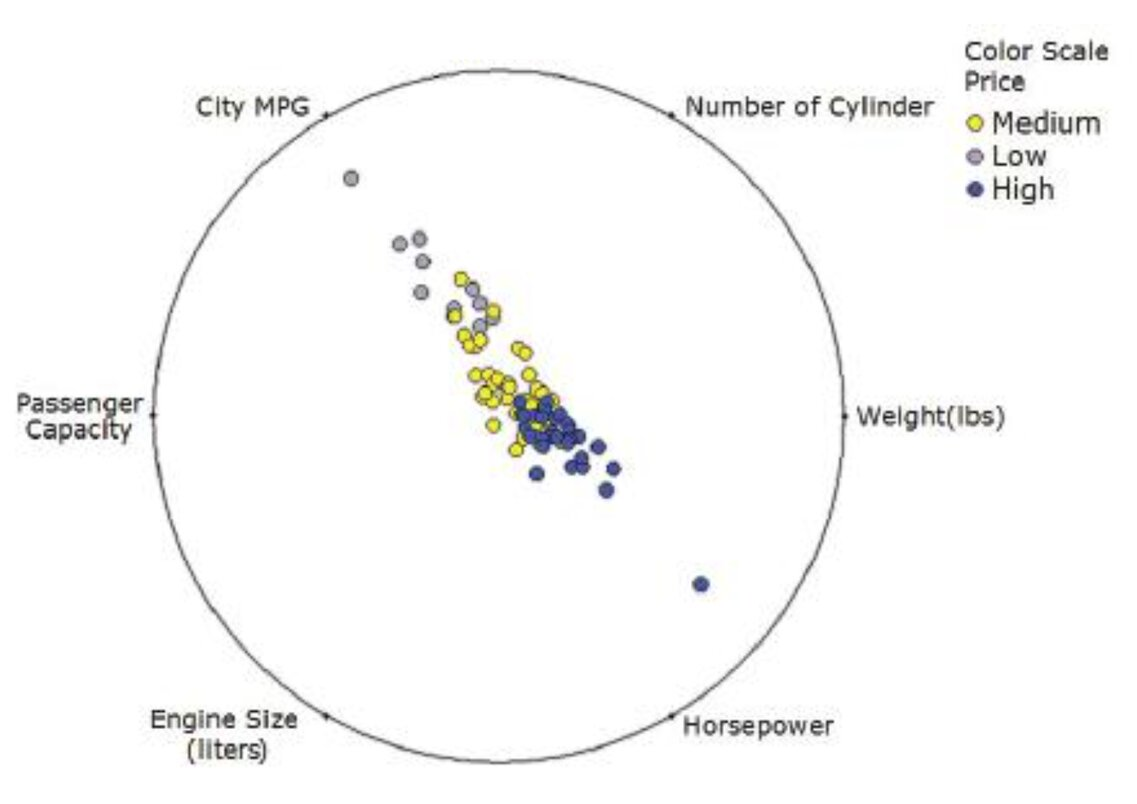
\includegraphics[width=12cm]{Gambar/datamobil-visual-titik.jpg}
    \caption{Visualisasi data spesifikasi mobil dengan teknik berbasis titik \cite{buku_visual}.}
    \label{fig:datamobil-visual-titik}
\end{figure}
Sebuah titik menyatakan proyeksi data yang terekam pada sebuah dimensi yang dapat diubah-ubah. Teknik visualisasi menggunakan titik untuk data individual mendefinisikan proyeksi data yang tepat dan representasi visual yang spesifik \cite{buku_visual}. Teknik berbasis titik yang paling sederhana adalah \textit{scatterplots}. Selain sederhana, teknik ini paling banyak digunakan untuk analisis data. Keberhasilan teknik ini tidak lepas dari kemampuan dasar manusia untuk mengamati posisi relatif pada ruang tertentu. \par
Teknik visualisasi berbasis titik dapat divariasikan dengan berbagai variabel visual, seperti warna yang dikombinasikan dengan modifikasi area dimensi. Pada Gambar \ref{fig:datamobil-visual-titik} diperlihatkan visualisasi data spesifikasi berbagai jenis mobil. Dari visualisasi tersebut telah dapat diperoleh seluruh informasi mengenai tingkat spesifikasi mobil yang dinyatakan dengan posisi relatif antar setiap tepi lingkaran. Harga dari setiap jenis mobil dapat diketahui dengan cepat dari kode warna yang digunakan. \par
\subsubsection{Teknik Berbasis Garis}
Dalam teknik visualisasi berbasis garis, setiap titik-titik yang menyatakan nilai tertentu dihubungkan menjadi sebuah garis lurus atau lengkung. Garis yang terbentuk tidak hanya memperkuat hubungan antar nilai data, tetapi juga menyampaikan informasi lain yang dapat dilihat melalui kemiringan, kelengkungan, persilangan, dan pola garis lainnya \cite{buku_visual}. Metode visualisasi berbasis garis paling banyak digunakan adalah diagram garis. Pada diagram garis, sumbu tegak menyatakan rentang nilai data, sedangkan sumbu mendatar menyatakan urutan tertentu. \par 
Pada kasus representasi data multivariabel, teknik berbasis garis dapat dikombinasikan dengan koordinat paralel. Pada Gambar \ref{fig:datamobil-visual-garis} diperlihatkan representasi data spesifikasi mobil dengan teknik berbasis garis menggunakan koordinat paralel. Ide dasar dari model visualisasi seperti ini adalah memetakan nilai data pada sebuah sumbu (vertikal ataupun horizontal) yang memiliki rentang nilai mewakili sebuah variabel tertentu, yang mana pada kasus ini setiap koordinat paralel mewakili spesifikasi mobil. Satu data tipe mobil direpresentasikan dengan menghubungkan garis pada setiap koordinat paralel yang posisi terhubungnya mewakili nilai tipe mobil untuk spesifikasi tersebut. \par  
Setiap teknik yang mengorientasikan koordinat secara horizontal dan/atau vertikal, terdapat pula teknik ekivalen yang mengorientasikan koordinat secara radial. Salah satu contoh penggunaan teknik berbasis garis dengan orientasi koordinat radial adalah diagram polar. Pada diagram polar setiap nilai data dipetakan pada koordinat polar. Seluruh nilai ini dihubungkan dengan garis yang membuat perubahan nilai data pada setiap arah dapat diamati dengan mudah. Teknik visualisasi menggunakan diagram polar banyak digunakan untuk memvisualisasikan data direktivitas, seperti yang ditunjukkan pada Gambar \ref{fig:diagramPolarBiola}, Gambar \ref{fig:contohPolarplotter}, dan Gambar \ref{fig:dipol}. \par
\begin{figure}[t!]
    \centering
    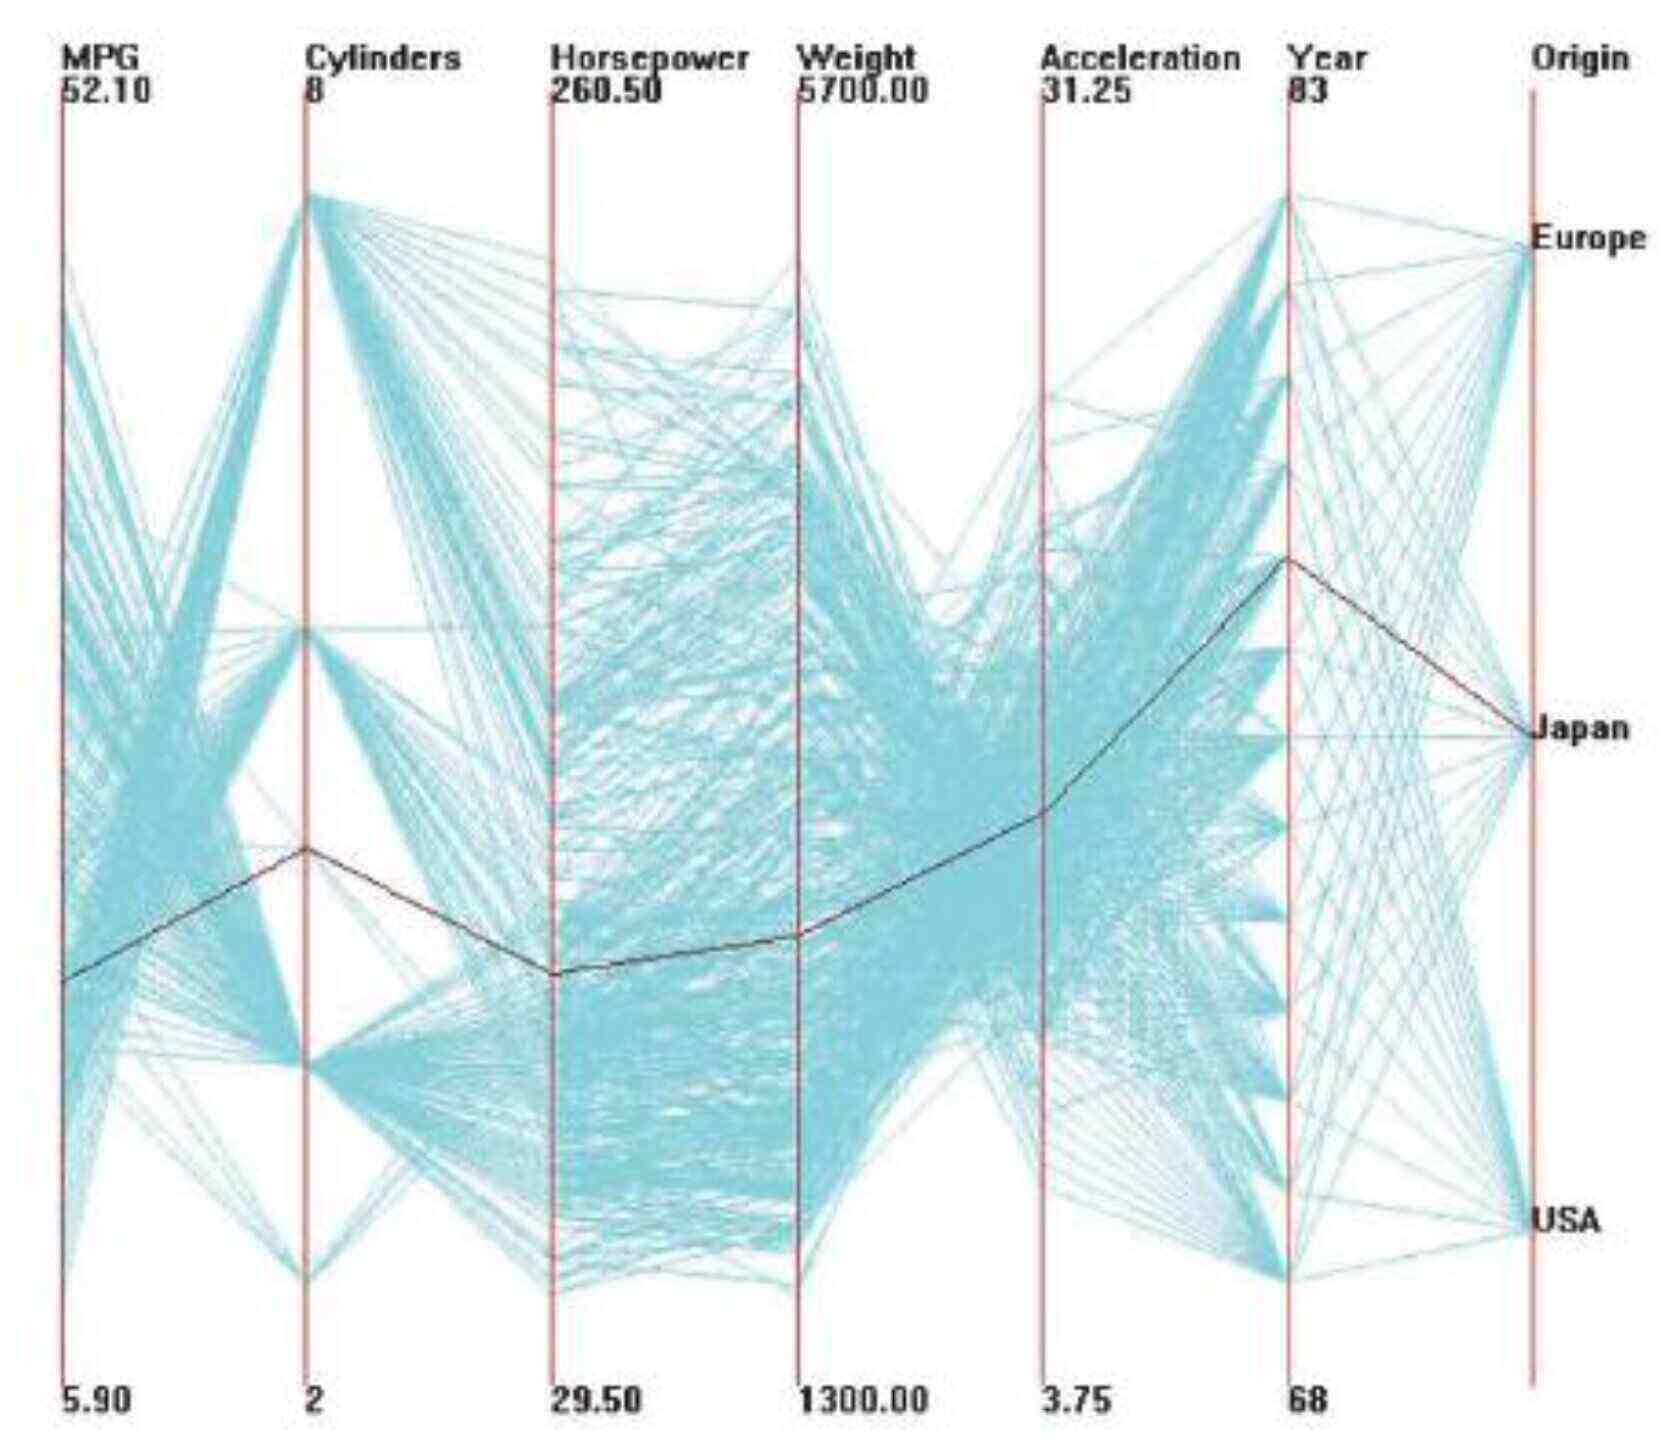
\includegraphics[width=10cm]{Gambar/datamobil-visual-garis.jpg}
    \caption{Visualisasi data spesifikasi mobil menggunakan teknik berbasis garis dengan 7-dimensi data pada koordinat paralel \cite{buku_visual}. Garis dengan warna yang disorot menandakan data individual yang dipilih.}
    \label{fig:datamobil-visual-garis}
\end{figure}
\subsubsection{Teknik Berbasis Area}
Pada teknik berbasis area, penyampaian informasi dilakukan dengan menggunakan bentuk yang berisi. Wilayah di dalam setiap bentuk objek visual digunakan untuk menyampaikan nilai data berdasarkan ukuran, bentuk, warna, ataupun variabel visual lainnya. Pada dasarnya kemampuan manusia untuk mengestimasi area secara akurat cukup buruk, tetapi teknik ini telah banyak dikembangkan dengan mengkombinasikan variabel visual yang lebih mudah diamati manusia. Pada umumnya, penggunaan teknik berbasis area tidak bertujuan untuk menyampaikan nilai data secara individual, melainkan untuk menyampaikan ringkasan atau distribusi nilai data. \par 
Teknik visualisasi berbasis area yang paling banyak digunakan seperti halnya \textit{scatterplots} dan diagram garis adalah diagram batang. Pada diagram batang, batang persegi panjang digunakan untuk menampilkan nilai numerik dari data. Penggunaan diagram batang dapat dengan mudah dipahami karena persepsi pandangan manusia lebih mudah membandingkan ukuran secara linear, baik vertikal maupun horizontal. Jika setiap bar membutuhkan penjelasan menggunakan teks, akan lebih baik jika teks dituliskan dengan arah horizontal. Keputusan paling krusial yang perlu diambil ketika mendesain diagram batang adalah menentukan berapa banyak batang yang diperlukan untuk menampilkan data. Jika visualisasi data bertujuan untuk menampilkan ringkasan dan sebaran data maka dapat digunakan histogram untuk menampilkan banyaknya kemunculan suatu nilai data. Jika rentang data cukup lebar, maka data perlu dibagi menjadi rentang-rentang yang lebih kecil. \par 
\begin{figure}[b!]
    \centering
    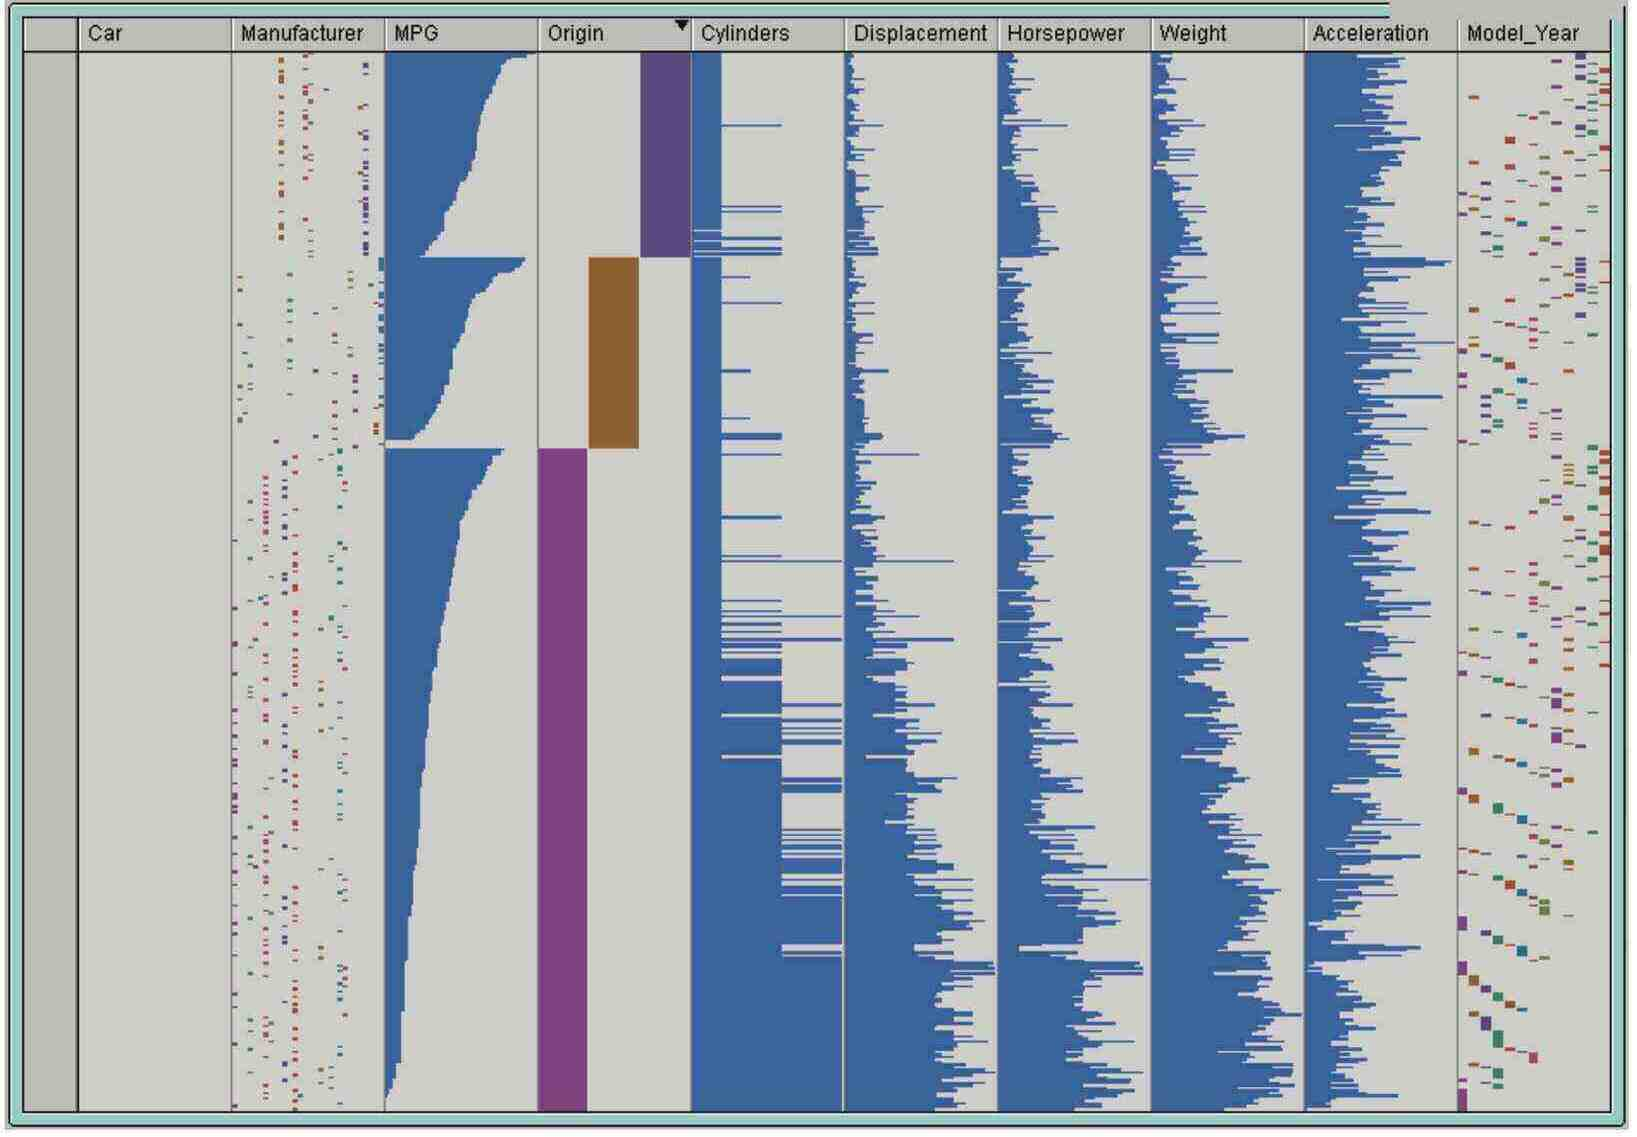
\includegraphics[width=10cm]{Gambar/datamobil-visual-area.jpg}
    \caption{Visualisasi data spesifikasi mobil menggunakan teknik berbasis area dengan lensa tabel \cite{buku_visual}.}
    \label{fig:datamobil-visual-area}
\end{figure}
Data multivariabel biasanya disimpan dalam bentuk tabel. Teknik berbasis area dapat diterapkan untuk meningkatkan efektivitas dari tampilan tabel, yaitu dengan menyajikan setiap nilai dari variabel ke dalam sebuah area tertentu seperti batang. Metode ini disebut sebagai lensa tabel \cite{buku_visual}. Pada Gambar \ref{fig:datamobil-visual-area} diperlihatkan representasi data spesifikasi mobil yang ditampilkan dalam bentuk lensa tabel. Pada lensa tabel, besarnya nilai pada spesifikasi dinyatakan dalam batang persegi panjang dengan variasi ukuran dan warna. Supaya sistem ini dapat berhasil, sistem harus dilengkapi dengan mekanisme level-detail yang baik, seperti menggeser dan memperbesar setiap batang pada sel tabel. \par 

%--- NEW
%--- SECTION

\section{Perancangan dan Pengembangan Produk}
Sebuah produk tercipta karena adanya kebutuhan penyelesaian masalah. Perancangan dan pengembangan produk adalah serangkaian aktivitas yang dimulai dari identifikasi peluang pasar dan berakhir pada proses produksi dan penjualan produk \cite{bukuUlrich}. Alasan utama sebuah produk dapat berhasil tentu karena adanya masalah yang perlu diselesaikan. Pada Bab \ref{pendahuluan} telah dipaparkan masalah yang dihadapi musisi dan pegiat \textit{bundengan}, sehingga proses identifikasi peluang pasar tidak diperlukan. Perancangan dan pengembangan produk kemudian berfokus pada beberapa kegiatan, yaitu identifikasi kebutuhan pengguna yang kemudian diterjemahkan menjadi spesifikasi konsep produk, lalu konsep tersebut perlu diuji kepada calon pengguna. Pada subbab ini akan dipaparkan bagaimana sebaiknya proses perancangan dan pengembangan produk dilakukan. \par 
\subsection{Identifikasi Kebutuhan Pengguna}
Pemahaman akan kebutuhan calon pengguna adalah kunci menuju kesuksesan sebuah produk \cite{bukuUlrich}. Oleh sebab itu, pada proses pengembangan sebuah produk proses identifikasi kebutuhan pengguna tidak boleh terlewatkan. Tujuan dari identifikasi kebutuhan pengguna ini antara lain adalah untuk memastikan produk berfokus pada kebutuhan pengguna, mengidentifikasi kebutuhan pengguna baik yang terlihat secara eksplisit maupun yang tersembunyi, mendapatkan alasan utama terkait spesifikasi produk, dan mendapatkan bayangan mengenai kegiatan selama proses pengembangan. Proses identifikasi ini umumnya terdiri dari empat tahapan, yaitu:
\begin{enumerate}
    \item Menggali data mentah dari calon pengguna.
    \item Menerjemahkan data mentah menjadi bentuk kebutuhan pengguna.
    \item Mengelompokkan kebutuhan pengguna ke dalam beberapa tingkatan prioritas.
    \item Refleksi hasil dan penentuan spesifikasi produk.
\end{enumerate}

Untuk mendapatkan data dengan kualitas terbaik, data tersebut harus diperoleh langsung dari calon pengguna. Metode paling umum yang digunakan untuk mendapatkan informasi dari pengguna adalah wawancara, diskusi grup, atau pengamatan terhadap produk yang sudah digunakan. Hasil akhir dari pengambilan data ini umumnya berupa pernyataan calon pengguna. Pernyataan-pernyataan ini kemudian diterjemahkan menjadi kebutuhan pengguna yang perlu ada dalam produk. \par 
Setiap pernyataan dari calon pengguna dapat diartikan menjadi banyak kebutuhan. Oleh sebab itu, digunakan sebuah panduan dasar yang dapat membantu menerjemahkan kebutuhan calon pengguna secara lebih efektif. Berikut ini adalah panduan menerjemahkan pernyataan calon pengguna menjadi kebutuhan \cite{bukuUlrich}.
\begin{enumerate}
    \item \textbf{Kebutuhan dinyatakan dalam bentuk "apa yang dapat dilakukan?" bukan "bagaimana melakukannya?".} Umumnya pengguna menggambarkan kebutuhan dalam bentuk implementasi sehari-hari, namun kebutuhan ini bukan tentang cara penyelesaian, melainkan apa yang harus diselesaikan.
    \item \textbf{Kebutuhan dinyatakan sedetail apa yang dinyatakan calon pengguna.} Jika calon pengguna mengungkapkan kebutuhan secara spesifik maka tingkat detil dari solusi yang dihadirkan juga harus spesifik.
    \item \textbf{Kebutuhan dinyatakan dalam frasa positif.} Proses eksekusi terhadap kebutuhan pengguna akan lebih mudah jika dinyatakan dalam frasa yang positif. Meskipun demikian, aturan ini tidak terlalu baku, karena terkadang ada kebutuhan yang memang perlu dinyatakan dalam frasa negatif seperti "Produk ini tidak memerlukan penggantian baterai".
    \item \textbf{Kebutuhan dinyatakan sebagai atribut produk.} Hal ini supaya spesifikasi produk dapat lebih mudah untuk ditentukan.
\end{enumerate}

Dari hasil interpretasi kebutuhan pengguna mungkin didapat banyak sekali daftar kebutuhan yang perlu diatasi oleh produk. Daftar kebutuhan tersebut perlu dikategorikan menjadi kebutuhan primer dan kebutuhan sekunder supaya proses penentuan spesifikasi produk dapat berjalan dengan baik. Pada produk yang kompleks, kebutuhan sekunder dapat dibagi lagi menjadi beberapa kebutuhan tersier. Hal pertama yang perlu dilakukan adalah mengeliminasi beberapa kebutuhan yang berulang kali muncul. Setelah tidak ada kebutuhan yang muncul lebih dari satu kali, daftar kebutuhan yang tersisa kemudian dikelompokkan menjadi kelompok kebutuhan yang lebih besar. Dengan pengelompokkan ini penentuan prioritas kebutuhan mana yang perlu diutamakan dapat dilakukan dengan lebih mudah. \par 
Sampai tahap ini proses identifikasi kebutuhan pengguna telah selesai. Hal yang perlu dilakukan adalah mengevaluasi apakah proses identifikasi ini telah berjalan dengan baik atau belum. Setelah proses evaluasi, daftar kebutuhan paling penting kemudian dapat digunakan untuk menentukan spesifikasi produk. \par 

%---

\subsection{Penetapan Spesifikasi Produk}
Kebutuhan pengguna yang telah diperoleh sebelumnya diungkapkan dalam bahasa "pengguna". Umumnya ungkapan tersebut bersifat subjektif seperti "mudah dipasang" atau "mudah digunakan". Hal ini akan sulit untuk diterapkan dalam proses perancangan dan rekayasa produk. Oleh sebab itu, perlu dilakukan penetapan sejumlah spesifikasi yang menguraikan secara rinci dan terukur apa yang dapat dilakukan produk \cite{bukuUlrich}. Proses penetapan spesifikasi produk terdiri dari tiga tahapan, yaitu pembuatan daftar metrik, pengumpulan informasi produk lain sebagai tolak ukur, dan penetapan target. \par
\subsubsection{Pembuatan Daftar Metrik}
Tahap pertama adalah membuat daftar ukuran kemampuan produk yang dapat memenuhi setiap kebutuhan pengguna. Ukuran kemampuan produk ini disebut sebagai metrik. Idealnya satu metrik dapat memenuhi satu kebutuhan pengguna, namun pada praktiknya hal ini seringkali tidak mungkin. Sebagai contoh, untuk pemenuhan kebutuhan "produk mudah dipasang" tidak hanya mempertimbangkan durasi waktu yang dibutuhkan untuk memasang produk, namun juga perlu memerhatikan kenyamanan dan keselamatan pengguna saat memasangnya. Terdapat beberapa aturan yang dapat dijadikan panduan dalam penyusunan daftar metrik, di antaranya adalah: \par
\begin{enumerate}
    \item \textbf{Metrik harus lengkap.} Ketika daftar metrik telah lengkap, pastikan tidak terdapat kebutuhan yang belum dipenuhi oleh sedikitnya satu metrik.
    \item \textbf{Metrik harus berupa variabel dependen, bukan independen.} Metrik harus mengindikasikan apa yang produk dapat lakukan, bukan bagaimana mencapai kebutuhan. Variabel dependen dapat berupa massa komponen, sedangkan variabel independen dapat berupa material penyusun komponen. Dengan fokus pada apa yang hendak dicapai, proses pengembangan produk dapat menggunakan langkah yang paling optimal.
    \newpage
    \item \textbf{Metrik harus praktikal.} Metrik yang dibuat harus dapat diaplikasikan pada proses pengembangan. Panduan ini mempertimbangkan keterbatasan waktu dan biaya pada proses pengembangan.
\end{enumerate}
\subsubsection{Pengumpulan Informasi Produk Kompetitif sebagai Tolak Ukur}
Supaya produk yang dikembangkan dapat bersaing dengan produk serupa di pasaran, perlu adanya analisis terkait spesifikasi produk yang sudah ada. Spesifikasi produk yang sudah ada dapat dijadikan tolak ukur kesuksesan produk yang akan dikembangkan. Proses tolak ukur dilakukan dengan membuat daftar perbandingan setiap metrik dari produk yang hendak dikembangkan dengan produk yang sudah ada di pasar. Dari daftar ini dapat diketahui spesifikasi seperti apa yang paling memenuhi kebutuhan pengguna sekaligus sesuai dengan batasan biaya dan waktu pada proses pengembangan. \par 
\subsubsection{Penetapan Target}
Pada tahap ini saatnya pengembang produk menentukan target spesifikasi produk berdasarkan informasi dan analisis yang didapat. Untuk memudahkan pengambilan keputusan, terlebih dahulu dapat dibuat dua versi target, yaitu target ideal dan target realistis. Target ideal adalah target dengan spesifikasi yang paling baik dan paling memenuhi kebutuhan pengguna. Target realistis adalah target yang memenuhi kebutuhan pengguna namun memiliki kualitas yang sesuai dengan keterbatasan waktu dan biaya pengembangan produk. Target realistis juga menyesuaikan harga jual produk terhadap daya beli calon pengguna di pasar tertentu. Target paling optimal yang dapat dikembangkan dapat diperoleh dari irisan kedua versi target ini. \par 


%---

\subsection{Uji Konsep Produk}
Dalam proses perancangan dan pengembangan produk, pengujian konsep produk kepada calon pengguna merupakan metode validasi pemenuhan kebutuhan calon pengguna \cite{bukuUlrich}. Jika terdapat lebih dari satu konsep produk, pengujian menjadi sarana penentuan konsep mana yang lebih baik untuk dilanjutkan. Selain itu, pengujian juga bertujuan untuk mengumpulkan informasi mengenai hal-hal yang perlu ditingkatkan dari konsep produk. Berikut adalah tujuh langkah pengujian konsep produk. \par 
\subsubsection{Penentuan Tujuan Uji} \label{sub-subBab:penentuan-tujuan-uji}
Pengujian konsep produk adalah kegiatan eksperimental \cite{bukuUlrich}. Ketika tujuan kegiatan eksperimental telah diketahui, akan lebih mudah dalam pemilihan metode yang efektif. Penentuan tujuan dilakukan dengan menuliskan beberapa pertanyaan yang harus terjawab setelah pengujian, seperti di antaranya
\begin{enumerate}
    \item Dari beberapa konsep alternatif, konsep manakah yang lebih baik?
    \item Apa yang perlu ditingkatkan supaya kebutuhan pengguna dapat tercapai?
\end{enumerate} 
\subsubsection{Pemilihan Populasi Survei}
Tujuan dilakukannya uji konsep produk didasari oleh populasi yang disurvei merefleksikan \textit{end-user} atau pengguna sesungguhnya dari produk tersebut \cite{bukuUlrich}. Oleh sebab itu, sebelum survei dilakukan, terlebih dahulu dipastikan apakah populasi yang dipilih benar-benar merepresentasikan pengguna yang ditargetkan. Selain itu, ukuran populasi yang disurvei juga menentukan tingkat representatif hasil survei. Semakin besar populasi survei, tingkat kepercayaan dalam pengambilan keputusan lanjutan juga akan semakin tinggi. Besar kecilnya ukuran populasi survei dapat ditentukan berdasarkan tujuan dilakukannya pengujian. Pada Tabel \ref{tab:ukuran-sampel} diperlihatkan beberapa alasan dalam memilih ukuran populasi. \par 
\begin{table}[h!]
    \centering
    \caption{Faktor-faktor penentu pemilihan ukuran sampel \cite{bukuUlrich}.}
    \begin{tabular}{m{0.7cm} m{6cm} m{6cm}}
        \hline
        \textbf{No} & \textbf{Sedikit sampel} & \textbf{Banyak sampel}\\
        \hline
        &&\\
        1. & Dilakukan pada awal & Dilakukan setelah\\
        & proses pengembangan & proses pengembangan\\
        &&\\
        2. & Bertujuan mendapatkan respon & Bertujuan mengetahui permintaan\\
        & secara kualitatif & secara kuantitatif\\
        &&\\
        3. & Pelaksanaan survei menghabiskan & Pelaksanaan survei relatif\\
        & banyak waktu dan biaya & cepat dan murah\\
        &&\\
        4. & Biaya produksi & Biaya produksi\\
        & tergolong rendah & tergolong tinggi\\
        &&\\
        5. & Perkiraan penilaian target & Perkiraan penilaian target\\
        & pasar relatif tinggi & pasar relatif rendah\\
        \hline
    \end{tabular}
    \label{tab:ukuran-sampel}
\end{table}
\subsubsection{Pemilihan Format Survei}
Berikut adalah beberapa format yang umum digunakan dalam pengujian konsep produk \cite{bukuUlrich}:
\begin{enumerate}
    \item \textbf{Interaksi tatap muka:} Pada format ini, pewawancara berkomunikasi secara langsung dengan responden. Format ini dapat dilakukan dengan mencari responden secara langsung di tempat umum atau merencanakan janji temu dengan responden.
    \item \textbf{Telepon:} Format ini serupa dengan wawancara tatap muka, namun akan terdapat beberapa keterbatasan dalam penyampaian konsep produk. Format wawancara melalui telepon lebih baik jika terlebih dahulu menentukan waktu dengan calon responden.
    \item \textbf{Surat elektronik:} Survei dengan format surat mengharuskan responden untuk merespon dalam format surat balasan yang lengkap. Oleh sebab itu, format ini hanya direkomendasikan jika antara pewawancara dan calon responden telah terbangun hubungan yang positif.
    \item \textbf{Internet:} Dengan menggunakan internet, pewawancara dapat membangun situs yang dapat menyediakan konsep secara visual. Responden dapat mengobservasi konsep dengan lebih baik lalu memberikan respon. Undangan menuju situs yang dibuat biasanya diberikan melalui surat elektronik.
\end{enumerate}

Pada masing-masing format, terdapat risiko terjadinya bias. Sebagai contoh, penggunaan format elektronik memungkinkan bias akibat perbedaan teknologi yang dimiliki setiap responden. Hasil dari survei dengan format elektronik akan buruk jika responden yang ditargetkan tidak memiliki sarana teknologi yang memadai. Untuk beberapa produk, tingkat kemampuan teknologi ini termasuk ke dalam profil pengguna produk \cite{bukuUlrich}. \par 
\subsubsection{Pengekspresian Konsep}
Konsep sebuah produk dapat dikomunikasikan dalam berbagai cara, di antaranya adalah sebagai berikut.
\begin{enumerate}
    \item \textbf{Deskripsi Verbal:} Umumnya deskripsi verbal adalah paragraf pendek atau poin ringkasan terkait konsep produk. Deskripsi ini dapat dibaca oleh responden ataupun dibacakan oleh orang yang bertugas melakukan survei.
    \item \textbf{Sketsa:} Sketsa pada umumnya berupa gambar garis yang menunjukkan perspektif produk.
    \item \textbf{Foto:} Fotografi digunakan untuk menyampaikan tampilan konsep produk. Foto produk yang masih dalam tahap pengembangan dapat dihasilkan dengan proses desain komputer.
    \item \textbf{Papan Cerita:} Papan cerita merupakan kumpulan gambar yang mengomunikasikan kegiatan yang melibatkan produk secara berurutan.
    \item \textbf{Video:} Gambar yang bergerak memungkinkan penyampaian konsep produk yang lebih dinamis. Bentuk dan cara penggunaan produk dapat dengan jelas dikomunikasikan.
    \item \textbf{Simulasi:} Umumnya simulasi adalah tiruan fungsi konsep produk yang diimplementasikan pada piranti lunak komputer.
    \item \textbf{Multimedia Interaktif:} Dengan menggabungkan video yang kaya akan komponen visual dengan simulasi interaktif, cara penyampaian konsep produk menjadi jauh lebih baik. Responden dapat mengamati informasi grafis maupun verbal melalui cara ini. Pengalaman yang dirasakan responden juga lebih baik karena cara ini melibatkan interaksi dua arah dengan responden.
    \item \textbf{Model Tampilan Fisik:} Model tampilan fisik atau figur secara jelas menampilkan bentuk dan tampilan dari produk. Seringkali terbuat dari kayu ataupun serat polimer yang kemudian diwarnai menyerupai produk.
    \item \textbf{Prototipe Produk:} Jika memungkinkan, penyampaian konsep menggunakan model kerja dapat sangat berguna untuk pengujian konsep produk. Meski begitu, penggunaan prototipe produk cukup berisiko. Responden akan menganggap prototipe adalah produk sebenarnya, sehingga responden akan beranggapan bahwa kekurangan dan disfungsional pada prototipe juga terdapat pada produk sesungguhnya.
\end{enumerate}

Ketika mengekspresikan konsep produk, promosi dan manfaat dari produk harus dinyatakan semenarik mungkin. Cara-cara penyampaian konsep produk tersebut sangat erat kaitannya dengan format survei yang dipilih. Setiap cara tidak selalu dapat digunakan pada semua format survei. Pada Tabel \ref{tab:bedaCara-bedaFormat} diperlihatkan format survei apa saja yang sesuai untuk masing-masing cara pengekspresian konsep produk. \par 
\begin{table}[t!]
    \centering
    \caption{Kesesuaian perbedaan format survei dengan setiap cara pengekspresian konsep produk \cite{bukuUlrich}.}
    \begin{tabular}{m{4cm} c c c c}
        \hline
        \textbf{}& \textbf{Telepon} & \textbf{Surat} & \textbf{Internet} & \textbf{Tatap Muka}\\
        & & \textbf{Elektronik} & \\
        \hline
        Deskripsi Verbal & $\bullet$ & $\bullet$ & $\bullet$ & $\bullet$ \\
        Sketsa & & $\bullet$ & $\bullet$ & $\bullet$ \\
        Fotografi & & $\bullet$ & $\bullet$ & $\bullet$ \\
        Papan Cerita & & $\bullet$ & $\bullet$ & $\bullet$ \\
        Video & & & $\bullet$ & $\bullet$ \\
        Simulasi & & & $\bullet$ & $\bullet$ \\
        Multimedia Interaktif & & &  & $\bullet$ \\
        Prototipe kerja & & &  & $\bullet$ \\
        \hline
    \end{tabular}
    \label{tab:bedaCara-bedaFormat}
\end{table}

\subsubsection{Pengukuran Respon Calon Pengguna}
Setelah mengomunikasikan konsep produk, pengguna akan diminta untuk mengisi formulir survei. Pertanyaan yang diajukan pada formulir survei harus sesuai dengan tujuan pengujian yang telah ditetapkan. Selain itu, untuk mengukur tingkat kegunaan produk digunakan skala numerik. Hal ini karena tingkat kegunaan suatu sistem hanya bisa didefinisikan pada sebuah konteks tertentu. Salah satu skala numerik yang dapat digunakan untuk pengukuran tingkat kegunaan sistem atau produk adalah SUS (\textit{System Usability Scale}) yang pertama kali diperkenalkan oleh Brooke pada tahun 1996 \cite{SUS}. Skala ini terdiri dari sepuluh pernyataan dengan lima tingkat jawaban. Jawaban berkisar dari nilai 1 = Sangat Tidak Setuju sampai dengan 5 = Sangat Setuju. Pada Tabel \ref{tab:susIndonesia} diperlihatkan daftar pernyataan SUS dalam adaptasi bahasa Indonesia. \par 
\begin{table}[t!]
    \centering
    \caption{SUS (\textit{System Usability Scale}) dalam bahasa Indonesia \cite{SUSIndonesia}.}
    \begin{tabular}{c m{11cm}}
        \hline
        \textbf{No.} & \textbf{Pernyataan}\\
        \hline
        1 & Saya berpikir akan menggunakan sistem ini lagi.\\
        2 & Saya merasa sistem ini rumit untuk digunakan. \\
        3 & Saya merasa sistem ini mudah untuk digunakan. \\
        4 & Saya membutuhkan bantuan dari orang lain atau teknisi dalam\\
        &  menggunakan sistem ini. \\
        5 & Saya merasa fitur-fitur sistem ini berjalan dengan semestinya. \\
        6 & Saya merasa ada banyak hal yang tidak konsisten (tidak serasi)\\
        &  pada sistem ini.\\
        7 & Saya merasa orang lain akan memahami cara menggunakan\\
        & sistem ini dengan cepat. \\
        8 & Saya merasa sistem ini membingungkan. \\
        9 & Saya merasa tidak ada hambatan dalam menggunakan sistem ini. \\
        10 & Saya perlu membiasakan diri terlebih dahulu sebelum \\
        &  menggunakan sistem ini.\\
        \hline
    \end{tabular}
    \label{tab:susIndonesia}
\end{table}
\subsubsection{Interpretasi Hasil}
Interpretasi hasil SUS adalah dengan total skor dari jawaban yang didapat. Sepuluh pernyataan pada SUS terdiri dari lima pernyataan positif dan lima pernyataan negatif. Pernyataan positif berada pada nomor ganjil, sedangkan pernyataan negatif berada pada nomor genap. Perhitungan total skor SUS didefinisikan dengan \cite{SUS}.
\begin{eqnarray}
    \text{Skor Ganjil}&=&\text{Nilai Jawaban}-1\\
    \text{Skor Genap}&=&5-\text{Nilai Jawaban}\\
    \Sigma\text{Skor}&=&\left(\Sigma\text{Skor Ganjil}+\Sigma\text{Skor Genap}\right)\times 2,5
\end{eqnarray}

Total skor dari SUS berkisar dari 0 sampai dengan 100. Total skor ini kemudian diterjemahkan menjadi kumpulan rentang sifat tertentu oleh Bangor, Kortum, dan Miller pada tahun 2009 \cite{SUSAdjective}. Pada Gambar \ref{fig:SUSAdjective} diperlihatkan perbandingan peringkat sifat dengan total skor dari SUS. Dengan skema pemeringkatan ini, setiap sistem yang diuji dapat disimpulkan kualitasnya. \par
\begin{figure}[t!]
    \centering
    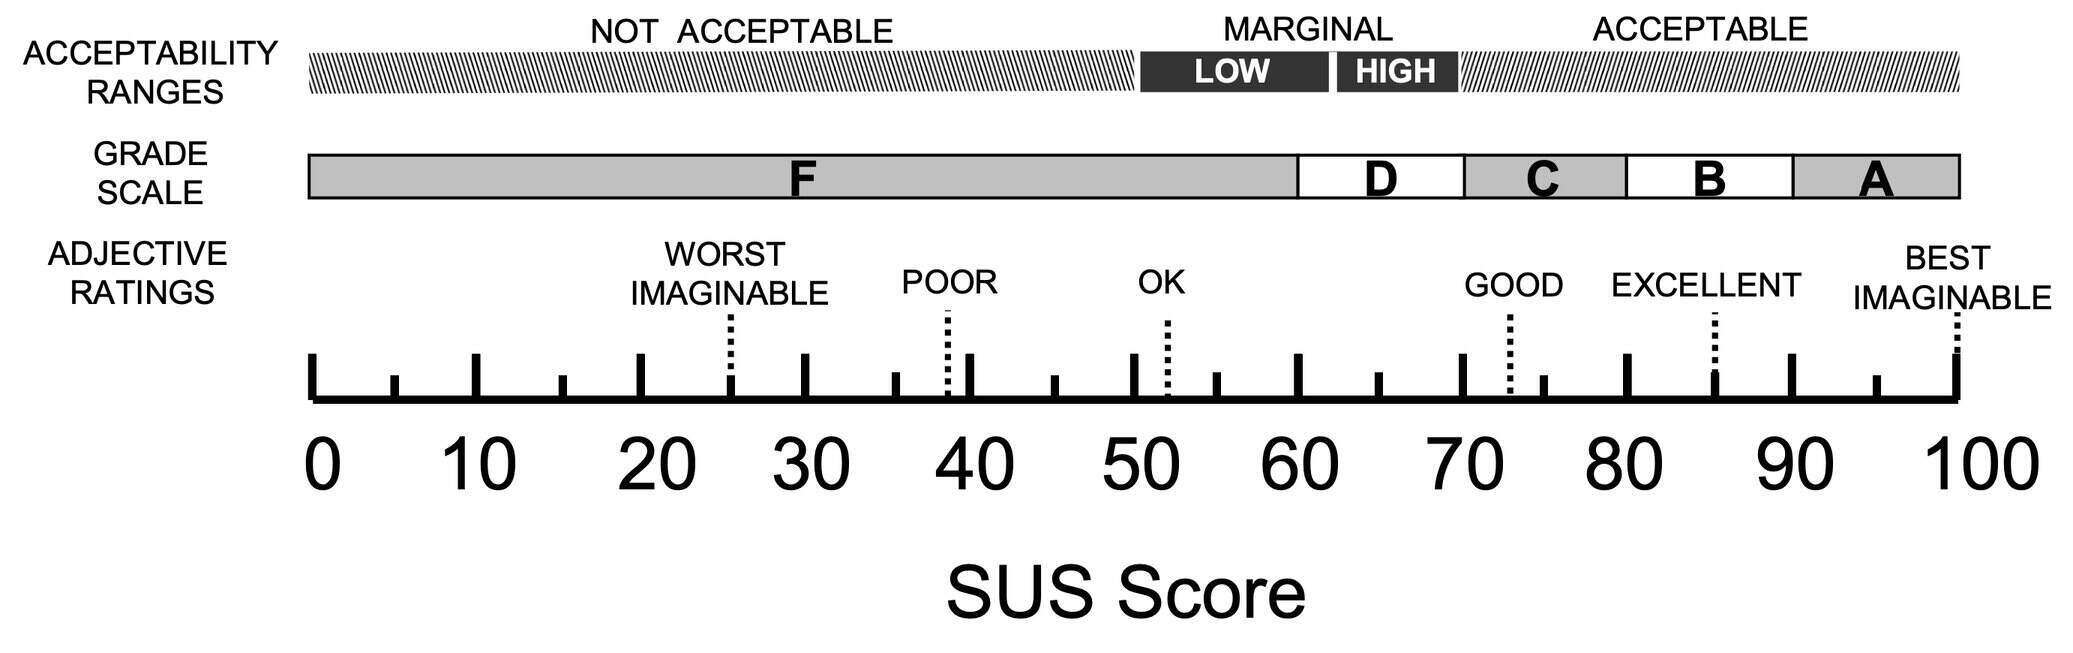
\includegraphics[width=14cm]{Gambar/adjective-sus.jpg}
    \caption{Perbandingan total skor SUS dengan peringkat sifat, peringkat nilai sekolah, dan rentang penerimaan \cite{SUSAdjective}.}
    \label{fig:SUSAdjective}
\end{figure} 

\subsubsection{Perencanaan Lanjutan Berdasarkan Hasil}
Tahap terakhir adalah perencanaan lanjutan. Dari hasil yang didapat, pihak pengembang produk dapat mulai menentukan bagaimana langkah selanjutnya untuk meningkatkan kualitas produk. Salah satu hal penting yang perlu direncanakan adalah peningkatan fungsional sistem sesuai kebutuhan yang diungkapkan calon pengguna pada survei. Selain itu, antusiasme calon pengguna yang telah terukur dapat menjadi acuan jumlah produk yang sebaiknya diproduksi untuk pertama kali. \par
